\documentclass[3p]{elsarticle} %preprint/3p

\usepackage{hyperref}

\journal{   }
\usepackage[T1]{fontenc}
\usepackage{amsmath} %added for maths environments (equation and align)
\usepackage{amssymb}
\usepackage{upgreek}
\usepackage{bm} %bold symbols by using \bm
\usepackage{mathtools, nccmath} %added for \xrightleftharpoons
\usepackage{stmaryrd} %math symbols
\usepackage{subcaption} %allowing for subcaptions and subfigures
\captionsetup[sub]{font=normalsize}%normalsize

\usepackage{algorithm} %added for algorithm box
\usepackage{algpseudocode}
\biboptions{sort&compress}

\usepackage[autostyle]{csquotes}
\MakeOuterQuote{"}

\bibliographystyle{elsarticle-num}

% slightly altering rules for figure placement to prevent full-page figures
\usepackage{placeins}
\renewcommand{\floatpagefraction}{.90}
\renewcommand{\topfraction}{.90}

\usepackage[capitalise, nameinlink]{cleveref}

\usepackage{todonotes} %added for todo notes
\let\oldtodo\todo
\renewcommand{\todo}[1]{\oldtodo[inline]{#1}}
%\renewcommand{\todo}[1]{\oldtodo[color=white!40,inline]{#1}}
\newcommand{\toask}[1]{\oldtodo[color=green!40, inline]{#1}}
\newcommand{\wrn}[1]{\oldtodo[color=red!40, inline]{#1}}

\usepackage{xcolor}
\usepackage{listings}
\usepackage{lstautogobble}
\usepackage[numbered]{matlab-prettifier}
\lstdefinestyle{mystyle}{
	numbers=left,
	numberstyle=\footnotesize,
	numbersep=8pt,
	style=Matlab-editor,
	tabsize=4,
	basicstyle=\ttfamily\footnotesize,
	numbersep=12pt,
	frame=none,
	autogobble=true
}
\newcommand{\CodeSnipU}[4]{\lstinputlisting[firstnumber=#2,firstline=#2,lastline=#3,style=mystyle,title={#4}]{../#1}}
\newcommand{\CodeSnip}[3]{\lstinputlisting[firstnumber=#2,firstline=#2,lastline=#3,style=mystyle,title={#1}]{../#1}}

\newcommand{\citeMe}{\href{https://doi.org/10.1016/j.electacta.2025.146203}{T Hageman, C Andrade, and E {Martinez-Pa{\~n}eda}. \textit{Corrosion of metal reinforcements within concrete and localisation of supporting reactions under natural conditions}. Acta Electrochemica} \citep{Hageman2025}}

\begin{document}
\pagenumbering{gobble}
\begin{frontmatter}
\title{ConcreteCorrosion: A C++ code to simulate natural corrosion of rebar within concrete.}

\author[1]{Tim Hageman \corref{mycorrespondingauthor}}
\cortext[mycorrespondingauthor]{Corresponding author}
\ead{tim.hageman@eng.ox.ac.uk}
\author[1]{Emilio Martínez-Pañeda}
\author[2]{Carmen Andrade}



\address[1]{Department of Engineering Science, University of Oxford, Oxford OX1 3PJ, UK}
\address[2]{International Center of Numerical Methods in Engineering (CIMNE), Madrid 28010, Spain}

\begin{abstract}
Documentation that accompanies the \textit{C++} code \href{https://github.com/T-Hageman/ConcreteCorrosion}{ConcreteCorrosion, available from \textcolor{blue}{here}}. This documentation explains how to compile the code, the usage of the implemented finite element framework, and highlight the main files.  The code allows the simulation of a corrosion pit with a supporting passivated surface, applied to corrosion of rebar within concrete. Specifically, it allows for an in-depth investigation of the locations of the cathodic and anodic reactions, under the requirement that the sum of these reaction currents acting on the complete rebar needs to be zero. If using (part of) this code, please cite \citeMe{}.  
\end{abstract}

\begin{keyword}
Corrosion, Electrochemistry, natural corrosion, Numerical simulation
\end{keyword}

\end{frontmatter}

\begin{figure}
	\centering
	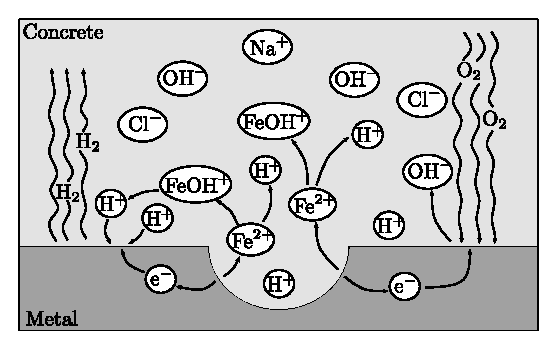
\includegraphics[width=10cm]{Fig1.eps}
	\caption{Overview of the system simulated using the presented C++ code}
\end{figure}

\newpage
\tableofcontents

\newpage
\pagenumbering{arabic}
\section{Introduction}

While reinforcements within concrete play a crucial role in bearing loads and enhancing the structural performance of buildings and infrastructure, they are inherently vulnerable to corrosion when exposed to aggressive environmental conditions. This susceptibility can lead to the development of internal stresses within the concrete matrix \citep{Page1982, Arya1996}, as the expansive nature of corrosion products exerts pressure on the surrounding material. As corrosion progresses, it contributes to the formation of local fractures \citep{Khan2014, Korec2023, Korec2024b}, which can compromise the load-carrying capacity of the structure. Additionally, the bond between the steel reinforcement and the adjacent concrete may deteriorate—a process known as de-bonding—which further diminishes the structural integrity \citep{Fang2004, Lee2002, Zhao2011, Michel2013}. Initially, the concrete’s internal environment is highly alkaline due to the presence of calcium hydroxide in the pore solution, which facilitates the formation of a protective passivation layer on the steel surface \citep{Page1982, Angst2011}. This layer effectively prevents corrosion under normal conditions. However, in the presence of chloride ions—often introduced through deicing salts, marine environments, or contaminated aggregates—the passivation film can be disrupted, allowing for the initiation of localized pitting corrosion \citep{Wang2021, Angst2019, Macdonald2021, Wang2013}.

Once a corrosion pit has formed, the chemical environment within the pit changes drastically. The hydrolysis of metal cations results in acidification of the local environment, further accelerating the corrosion process. Even if the original source of chloride ions is later removed, repassivation is unlikely due to the persistently low pH conditions inside the pit \citep{Pourbaix1975, Taylor2018a, Li2021a, Turnbull1983, Pickering1972}. This localized breakdown of the protective layer means that anodic and cathodic reactions occur in spatially separated regions on the steel surface, with the anodic sites (where metal dissolution occurs) being particularly confined and aggressive. Surrounding these active corrosion zones, cathodic reactions consume the electrons generated by the anodic dissolution, thereby maintaining the electrochemical circuit and influencing the steel’s overall potential \citep{Hoar1967, Galvele1981, Frankel2017, Frankel1990, Nguyen2021}. Over time, the progressive growth of corrosion pits reduces the effective cross-sectional area of the reinforcing bars, thereby compromising their mechanical performance and increasing the likelihood of structural failure. Furthermore, the accumulation and expansion of corrosion products within the concrete create significant internal tensile stresses. These stresses induce cracking and spalling of the concrete cover, which not only weakens the structure but also exposes more steel surface to corrosive agents. As a result, the durability and service life of reinforced concrete structures are substantially diminished \citep{korec2024phase}.

Therefore, it is crucial to establish the changes in the local environment, the range over which these changes are induced, and how long these changes are being sustained by the presence of a corrosion pit under realistic circumstances. This code focusses on these aspects, assuming a constant corrosion pit geometry, and resolving how the corrosion currents change over time. It also incorporates the requirement that these corrosion currents are supported by hydrogen and oxygen evolution reactions. Here, we present the C++ implementation of a new computational model to estimate the corrosion of reinforcements within concrete, under the requirement that the corrosion current is fully supported by hydrogen and oxygen evolution reactions. This requirement emulates natural corrosion, where the rebar is fully isolated from any external current and potential sources. As this creates a direct link between the corrosion rate and the cathodic reaction rates, this model allows for in-depth analysis of the processes causing corrosion in natural conditions. We furthermore do not impose any specific reaction areas, rather letting the computational model resolve these by itself, to study which areas of the rebar partake in the electrochemical reactions. 

These two important and novel model features allow us to gain new physical insight and answer the pressing questions formulated above. In the remainder of this documentation, we will first describe how to install and run the simulation code, followed by a description of the mesh generation and the input files. We will then describe the models implemented in the code, and finally describe the output files generated during the simulation. For a full description of our model, we refer to \citeMe{}.


\subsection{Installation}

\subsubsection{Required external libraries}
The simulation code has been developed to work directly in ubuntu, or within windows using WSL \citep{mattwojo}. A script is included which installs all required libraries, \textit{Install\_Libs.sh}. While it can be directly run to install all libraries at once, it is recommended that the contents is run line-by-line by copying it into the terminal. This allows for easier debugging in case of errors. The script installs the following libraries:

\noindent \textbf{Intel OneMKL} \citep{oneMKL} is used for its linear matrix solvers (and used by PETSc).\\
\textbf{Eigen} \citep{eigen} is used for small matrix and vector mutliplications.\\
\textbf{RapidJSON} \citep{rapidjson} is used for reading the input files.\\
\textbf{VTK} \citep{VTK} is used for visualisation during simulations.\\
\textbf{Highfive} \citep{HighFive} is used to write output files in the HDF5 format.\\
\textbf{PETSc} \citep{PETSc} is used for its implementation of parrallel (MPI) matrices and vectors (and their associated solvers).

Most of the above libraries are easy to install. However, for PETSc care needs to be taken to enable support for C++, link to the Intel MKL library, and enable support for HDF5. This is enabled through the command:
\CodeSnipU{Install_Libs.sh}{83}{84}{Install\_Libs.sh}

In addition to the environmental variables set by OneMKL and PETSc (\$PETSC\_DIR, \$ PETSC\_ARCH, \$MKLROOT), an additional environmental variable is used in the cmake files to locate the other libraries, \$LIBRARY\_DIR, which should point to the parent folder that contains the eigen, rapidjson, and Highfive folders. 

\subsubsection{Compiling}
The code makes uses of cmake to create appropriate makefiles. To compile the code, first run cmake using \textit{cmake .} from the base directory, after which the code itself can be compiled using \textit{make} (or \textit{make -j 56} to compile in parrallel). 


\subsection{Basic usage}
\label{sec:usage}
Once compiled, the code can be run using \textit{./ConcreteCorrosion <inputfile>} to run on a single core, or \textit{mpirun -n <number of cores> ./ConcreteCorrosion <inputfile>} to run in parallel. Example input files are included within the folder \textit{TestCases/Electrochemistry}. Running the code using the example file will print the progress of the simulation to the terminal, and open several plots showing the state of the system, with an example shown in \cref{fig:Results}. Note that while the simulation considers a three-dimensional domain, plots are only produced on 2D edges of the domain. The code will also save the results to a file, which can be visualised using the \textit{PlotData.m} matlab script. 

\begin{figure}
	\centering
	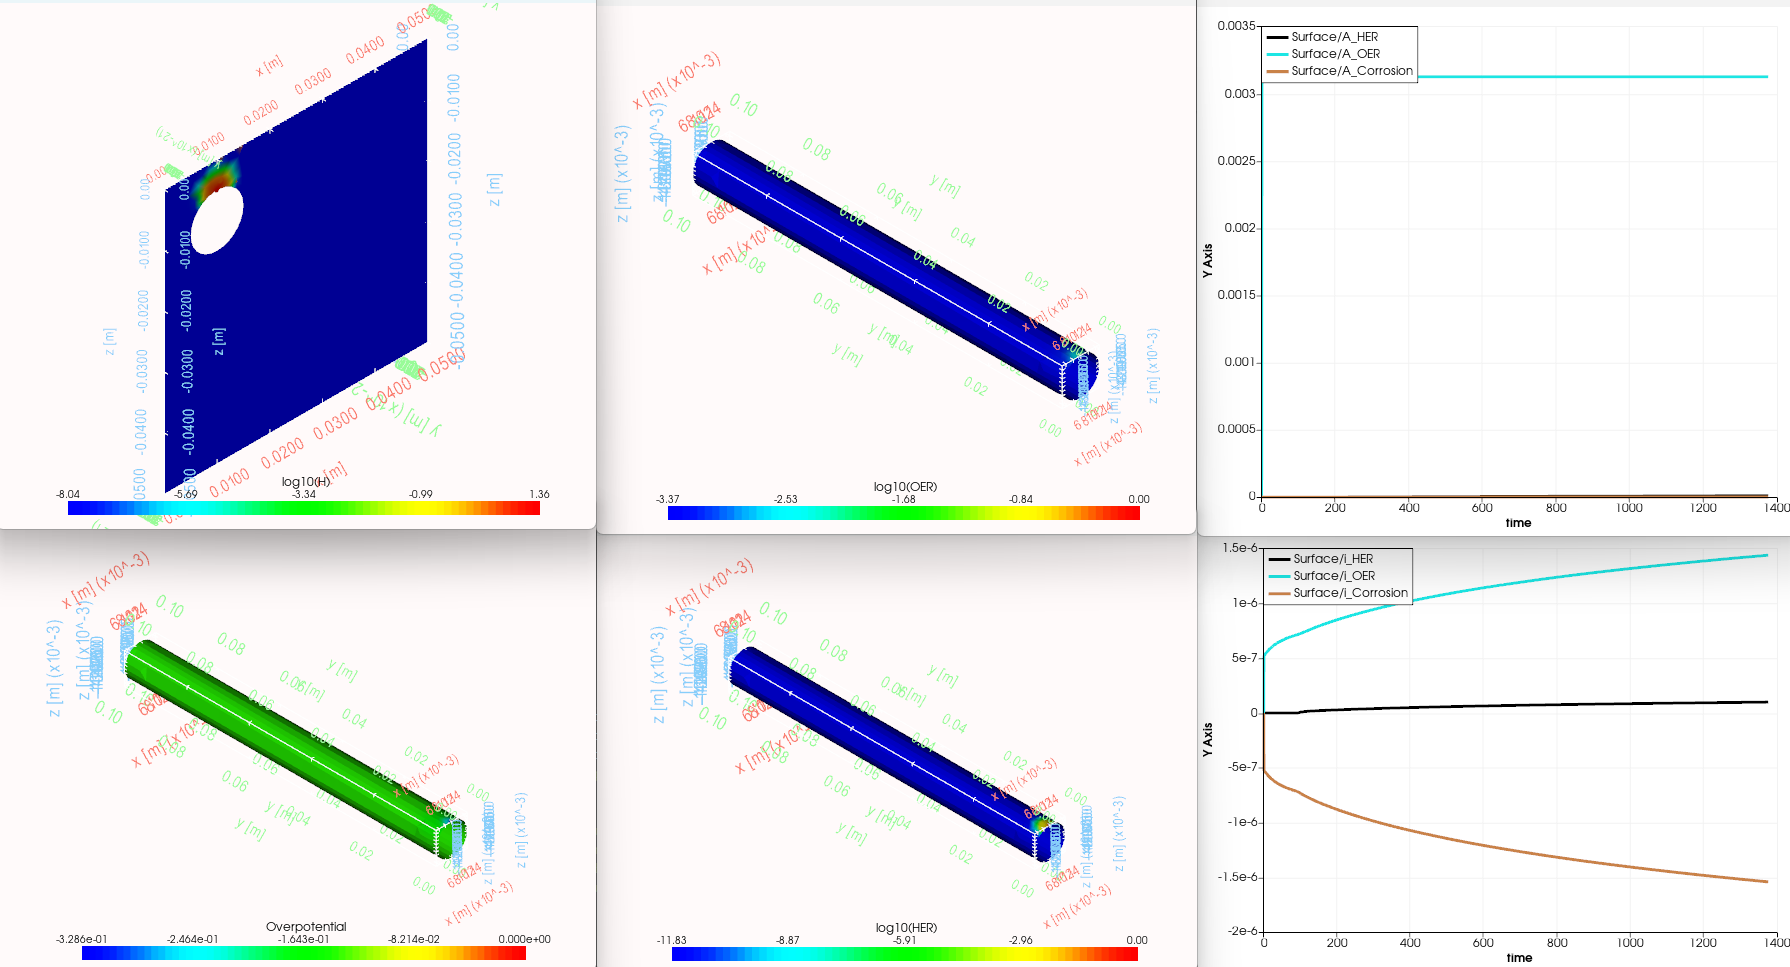
\includegraphics[width=14cm]{Screenshot.png}
	\caption{Example of the plots produced during the simulation. The top left shows the $\text{H}^+$ concentration, the top middle the oxygen evolution reaction current, top right the areas involved in the surface reactions. The bottom left shows the overpotential, middle the hydrogen evolution reaction rate, and the bottom right shows the reaction rates for each surface reaction.}
	\label{fig:Results}
\end{figure}

\subsection{Input Files}
The input file contains the following sections:

\subsubsection{Mesh}
\CodeSnipU{TestCases/ElectroChemistry/Test_ElectroChem.json}{11}{15}{TestCases/ElectroChemistry/Test\_ElectroChem.json}
which defines the file to use as mesh (see also \cref{sec:mesh}), indicates that the mesh is 3D, and sets the number of integration points per dimension to 3 (e.g. 3x3x3 integration points for volume elements, 3x3 for surface elements). 

\subsubsection{Chemical species}
Next, the chemical species are defined via:
\CodeSnipU{TestCases/ElectroChemistry/Test_ElectroChem.json}{16}{25}{TestCases/ElectroChemistry/Test\_ElectroChem.json}
First defining the names of the chemical species present, and then defining their diffusivity (D), ionic charge (z, this can be set to zero), the initial concentration (C0), and whether the diffusivity and concentration should be corrected for the water saturation (Aqueous). Note that the amount of degrees of freedom is automatically adapted to match the number of species declared here. As such, extra species can be freely added or removed within needing to update the simulation code itself.

\subsubsection{Bulk Reactions}
Chemical reactions occurring within the bulk are defined by:
\CodeSnipU{TestCases/ElectroChemistry/Test_ElectroChem.json}{63}{85}{TestCases/ElectroChemistry/Test\_ElectroChem.json}
First defining names for all reactions that are considered in the bulk (this list can be expanded to include mode reactions), and then defining the parameters for each individual reaction. This includes defining whether the reaction is assumed to be either solved as a dynamic or equilibrium reaction, the species involved in the reaction (this can be left empty if water or other unresolved species are involved), and their respective stoichiometric coefficients. For equilibrium reactions, this furthermore requires setting the equilibrium constant (K), and a dummy rate k\_dummy to be chosen high enough to enforce equilibrium. For dynamic reactions, the forward and backward rates k are defined. Finally, a flag used to indicate whether a lumped integration scheme should be used to stabilize the reactions is included \citep{Hageman2023a}. 

\subsubsection{Surface Reactions}
Surface reactions are defined in a similar way as bulk reactions:
\CodeSnipU{TestCases/ElectroChemistry/Test_ElectroChem.json}{97}{112}{TestCases/ElectroChemistry/Test\_ElectroChem.json}
Defining the type of surface reaction, the reference reaction currents i0, the charge transfer coefficient alpha, the equilibrium potential E\_eq, the species and electrons involved as input and output, and the surface this reaction occurs on (used by later modules).

\subsubsection{Degrees of freedom}
This section defines the degree of freedom names (these should include the species declared earlier), using ePot to declare the electrolyte potential, and Em to declare the metal potential:
\CodeSnipU{TestCases/ElectroChemistry/Test_ElectroChem.json}{146}{149}{TestCases/ElectroChemistry/Test\_ElectroChem.json}
While it is possible to declare that species are resolved in a staggered manner (by setting DofStep to different valeus), this will cause convergence issues and is not recommended. 

\subsubsection{Solver settings}
The solver settings are defined in the following section:
\CodeSnipU{TestCases/ElectroChemistry/Test_ElectroChem.json}{150}{166}{TestCases/ElectroChemistry/Test\_ElectroChem.json}
Defining the maximum amount of Newton-Raphson iterations (max\_it), the convergence criteria used (convCrit, with the three components corresponding to a criterion based on the norm of concentrations, forces, and energy respectively), whether a line search algorith is used, and which linear solver is used to solve the coupled system of equations (either \textit{Pardiso}, \textit{MUMPS}, or \textit{GMRES}). Finally, this section declares that the degrees of freedom are initialised consistent with the C0 declared in the species section.

\subsubsection{Time discretisation options}
This section declares the time discretisation options:
\CodeSnipU{TestCases/ElectroChemistry/Test_ElectroChem.json}{167}{173}{TestCases/ElectroChemistry/Test\_ElectroChem.json}
detailing the initial time increment dt, the rate at which this time increment increases (dtGrow), the maximum time increment (dtMax), and the total duration of the simulation (tmax). This also declares how often output files should be saved, through the outputN parameter. 

\subsubsection{Outputs}
The output section defines the variables to be written to the output files for later post-processing/visualisation:
\CodeSnipU{TestCases/ElectroChemistry/Test_ElectroChem.json}{174}{190}{TestCases/ElectroChemistry/Test\_ElectroChem.json}

\subsubsection{Physics models}
This section declares the models and boundary conditions to be used (see also \cref{sec:models} for more details):
\CodeSnipU{TestCases/ElectroChemistry/Test_ElectroChem.json}{191}{229}{TestCases/ElectroChemistry/Test\_ElectroChem.json}
with the Name field detailing which physics model to use. 

For the NernstPlanck model, it also requires the element groups for the concentrations and electrolyte potential to be defined, the porosity of the concrete to be set (Porosity), the tortuity coefficient (PorosityFactor), the saturation and saturation limits (Sw and S\_irr respectively), the exponent used for the saturation-diffusion relation (SatFactor), and if any numerical stabilisation is used. 

For the Surface reactions, this requires setting the element groups that represent the surface. Additionally, for each area indicated as surface, SurfaceReactions needs to be set to define which reactions occur on this surface (using the same names as used when these reactions were first defined). This model also allows toggling the charge conservation on and off, and sets a threshold value (solely used for post-processing) to indicate when a surface reaction is considered to be negligible (ActiveCurrent\_Threshold). This threshold is used to calculate the areas associated with each reaction, but is not used to impose any constraints on the reaction rates themselves.

For the boundary condition models, this requires setting which species are imposed by the boundary condition, and what the electric potential at the boundary is.

\subsubsection{Visualisation}
Finally, during the simulation, optional plots are produced as defined in visualisation: 
\CodeSnipU{TestCases/ElectroChemistry/Test_ElectroChem.json}{230}{237}{TestCases/ElectroChemistry/Test\_ElectroChem.json}
Indicating the degree of freedom to plot, the surface where to plot this for, and how often the plots are updated. Note that, for computational efficiency, the plots produced during the simulation are non-interactive. 


\section{Mesh Generation}
\label{sec:mesh}
Meshes used for the simulations are generated in MATLAB before running the simulation itself. AN example of mesh generation is given in \textit{TestCases/ElectroChemistry/Mesh/Beam.m}, which generates the mesh used for all the results in our paper. 

The initial geometry is defined as a .stl file, and imported into MATLAB via 
\CodeSnip{TestCases/ElectroChemistry/Mesh/Beam.m}{31}{32}
This geometry is then used to create a basic mesh, defining the maximum element sizes in the pit, and on the surface of the rebar:
\CodeSnip{TestCases/ElectroChemistry/Mesh/Beam.m}{37}{37}
To make this mesh suitable for finite element simulations, separate element groups are extracted for the interior elements and the boundaries:
\CodeSnip{TestCases/ElectroChemistry/Mesh/Beam.m}{47}{49}
Finally, this mesh is partitioned to be compatible with the required number of cpu cores, and saved to a file:
\CodeSnip{TestCases/ElectroChemistry/Mesh/Beam.m}{116}{122}
Running this MATLAB script also plots the mesh, producing the figure shown in \cref{fig:Mesh}.

\begin{figure}
	\centering
	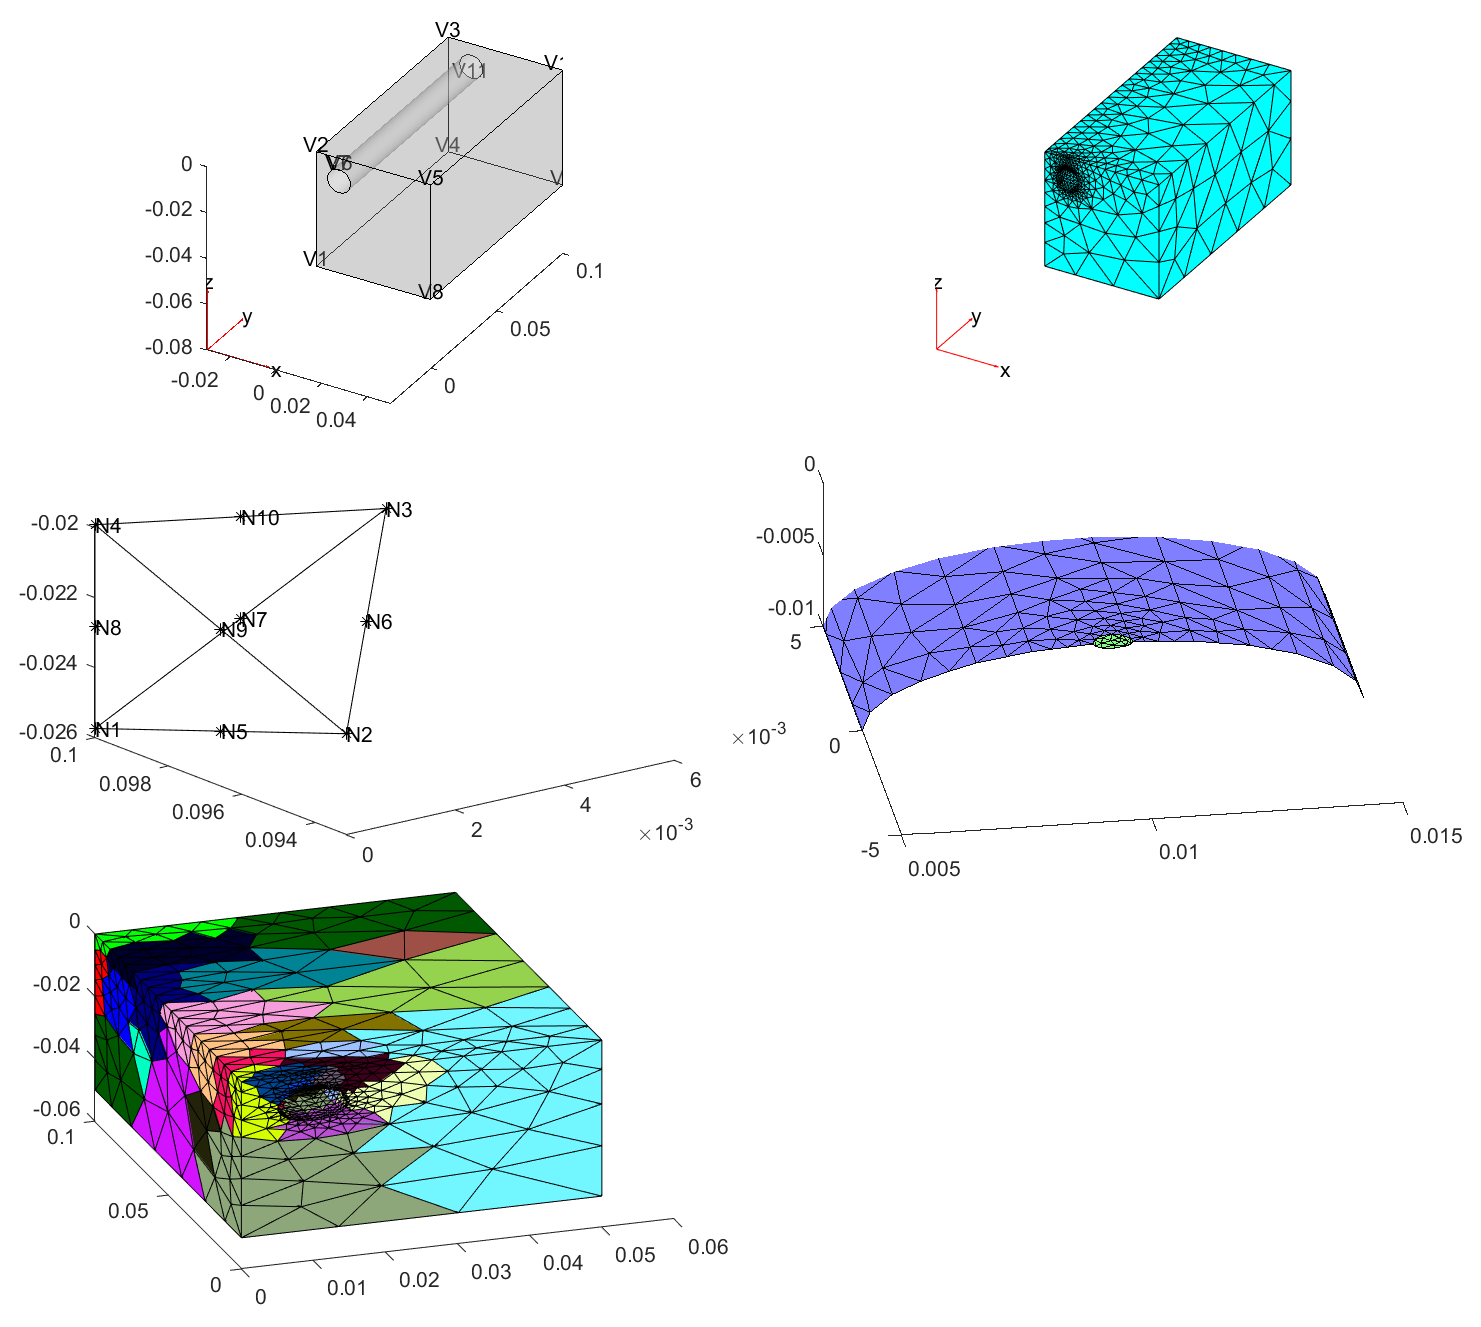
\includegraphics[width=14cm]{MeshFig.eps}
	\caption{Example of a mesh generated using the MATLAB script \textit{Beam.m}. The figure shows the geometry (top left), generated mesh (top right) and a close-up of the mesh near the corrosion pit (middle right), the node numbering for volume elements (middle left), and how the mesh is partitioned and distributed between cpu cores (bottom).}
	\label{fig:Mesh}
\end{figure}

\subsection{Mesh file format}
The saved output file has the following entries:
\begin{itemize}
	\item NCores: number of CPU cores this mesh is generated for
	\item nodes: 3xn matrix containing the coordinates of all the nodes
	\item nodegroupnames: Names for all node groups used
	\item nodegroups/<name>: Vector containing the indices of all nodes associated with this groups
	\item elementgroupnames: Names for all element groups used
	\item elementgrouptypes: Types of all element groups used, using \textit{T3\_10B} to indicate tetrahedral, quadratic, Bernstein volume elements, and \textit{T2\_6B} to indicate triangular, quadratic, Bernstein surface elements
	\item elementgroups/<name>: mxn matrix containing the nodes m associated with each element n. 
	\item <core>/noderange: Indicates the node ownership range of this cpu core. 
	\item <core>/ghosts: Indicates the nodes which are not owned by the core, but are required to be synced with neighbouring cores. 
	\item <core>/nodegrouprange: Vector indicating the start and end for each nodegroup owned by this cpu core
	\item <core>/Haselems: Vector indicating whether this core contains any elements for each elementgroup
	\item <core>/elemrange: Vector indicating the start and end for each elementgroup owned by this cpu core
\end{itemize}

\section{Summary of included models}
\label{sec:models}

\subsection{Nernst-Planck equations}
This model is implemented in \textit{Models/Electrochemistry/NernstPlanck.cpp}. It implements the conservation of chemical species using the Nernst-Planck equation:
\begin{equation}
    S^*_\pi \phi \dot{C}_\pi +\bm{\nabla}\cdot\left(-D_\pi^{\text{eff}} \bm{\nabla}C_\pi\right)+\frac{z_\pi F}{RT}\bm{\nabla}\cdot\left(-D_\pi^{\text{eff}} C_\pi \bm{\nabla}\varphi\right) + \phi S^* R_\pi = 0 \label{eq:massconserv}
\end{equation}
where $S^*$ is the water saturation, $\phi$ the porosity, $C_\pi$ is the concentration of species $\pi$, $D_\pi^{\text{eff}}$ is the effective diffusivity of species $\pi$, $z_\pi$ is the ionic charge of species $\pi$, $F$ is Faraday's constant, $R$ is the universal gas constant, $T$ is the temperature, and $\varphi$ is the electric potential. The term $R_\pi$ represents the reaction rate of species $\pi$. The effective diffusivity is defined in terms of the saturation and porosity as \citep{Tartakovsky2019, Ghanbarian2013}:
\begin{equation}
    D_\pi^{\text{eff}} = \phi^{3/2} D_\pi \left(\frac{S_\text{w}-S_\text{irr}}{1-S_\text{irr}}\right)^2 \label{eq:Deff}
\end{equation}
where the exponents $3/2$ and $2$ correspond to the factors set in the input file for \textit{PorosityFactor} and \textit{SatFactor} respectively. 

\cref{eq:massconserv} is combined with the electroneutrality condition:
\begin{equation}
    \sum_\pi \phi z_\pi C_\pi = 0 \label{eq:electroneutrality}
\end{equation}
with this condition allowing the electrolyte potential $\varphi$ to be obtained, implicitly taking into account the local diffusivity and ion concentrations (and thus the local conductivity) \citep{Feldberg2000}. 

For the volume reactions included in the $R_\pi$ term, this considers dynamic reactions and equilibrium reactions, with their implementation performed in \textit{Models/ElectroChemistry/Reactions.cpp}. For the dynamic reactions, the reaction rates are defined as:
\begin{equation}
	R = k_f \prod_{\pi_i} \frac{C_{\pi_i}}{C_\text{ref}} - k_b \prod_{\pi_j} \frac{C_{\pi_j}}{C_\text{ref}} \label{eq:dynamic}
\end{equation}
where $k_f$ and $k_b$ are the forward and backward reaction rates, $\pi_i$ and $\pi_j$ are the species involved in the forward and backward reactions respectively, and $C_\text{ref}$ is a reference concentration. Based on this rate, the reaction term is then obtained as:
\begin{equation}
	R_\pi = \frac{R}{n_\pi} \label{eq:reactionrate}
\end{equation}
where $n_\pi$ is the stoichiometric coefficient of species $\pi$ in the reaction.

For equilibrium reactions, the reaction rate is defined as:
\begin{equation}
	R = k_\text{dummy} \left(K\prod_{\pi_i} \frac{C_{\pi_i}}{C_\text{ref}} - \prod_{\pi_j} \frac{C_{\pi_j}}{C_\text{ref}}\right) \label{eq:equilibrium}
\end{equation}
where $K$ is the equilibrium constant, and $k_\text{dummy}$ is a dummy rate used to enforce equilibrium. The reaction term is then obtained in the same way as for dynamic reactions, using \cref{eq:reactionrate}.

\subsection{Surface reactions \& charge conservation}
The surface reactions and charge conservation condition are implemented in \textit{Models/Electrochemistry/SurfaceReactions.cpp}. These surface reactions are defined through the Butler-Volmer equation, giving the reaction current as:
\begin{equation}
	i = i_0 \exp\left(\frac{\alpha z F \eta}{RT}\right)K\prod_{\pi_i} \frac{C_{\pi_i}}{C_\text{ref}} - i_0' \exp\left(-\frac{(1-\alpha) z F \eta}{RT}\right)\prod_{\pi_j} \frac{C_{\pi_j}}{C_\text{ref}}  \label{eq:ButlerVolmer}
\end{equation}
with $i_0$ and $i_0'$ the reference reaction currents, $\alpha$ the charge transfer coefficient, $z$ the number of electrons involved in the reaction, and $\eta$ the overpotential. From this reaction current, the species flux at the metal surface is given by:
\begin{equation}
	\nu_\pi = \frac{i\;n_\pi}{z_\pi F} \label{eq:flux}
\end{equation}
Finally, this model also implements the charge conservation condition, which is used to ensure that the sum of all anodic and cathodic reactions on the surface is zero. This is done by solving the following equation:
\begin{equation}
	\int_\Gamma \sum_\pi i_\pi \;\text{d}\Gamma = 0 \label{eq:chargeconservation}
\end{equation}
with this constraint being imposed to allow the metal potential to change over time. 

\subsection{Boundary conditions}
The final model included is responsible for adding the boundary conditions, implemented in \textit{Models/Electrochemistry/EChemConstraints.cpp}. This model adds boundary conditions based on the C0 values set in the input file to the surface the boundary condition is applied to. The set boundary conditions are eliminated from the tangent matrix and force vectors through  allocation matrices $\bm{C}_\text{con}$ and $\bm{C}_\text{uncon}$, reordering the system into a constrained and unconstrained part. This allows the constrained system to be solved as:
\begin{equation}
	\bm{C}_\text{uncon}^T \bm{K} \bm{C}_\text{uncon} \mathbf{y} = -\left(\bm{C}_\text{uncon}^T\bm{f}+\bm{C}_\text{uncon}^T \bm{K} \bm{C}_\text{con}\mathbf{c}\right)
\end{equation}
with the values of the boundary constraints contained in the vector $\mathbf{c}$. After solving, the state vector is then incremented through:
\begin{equation}
	\mathbf{x}^\text{new} = \mathbf{x}^\text{old} + \bm{C}_\text{uncon}\mathbf{y} + \bm{C}_\text{con}\mathbf{c}
\end{equation}


\section{Output files and post-processing}

\subsection{Output files}
The simulations will output three kinds of files to the output folder, a mesh file, a series of results files, and a temporal data file, all of which use the HDF5 file format. The mesh file contains the mesh used for saving the outputs, structured as (where ElementGroup is either Pit/Bar/Interior):
\begin{itemize}
	\item <ElementGroup>/X: 3xn matrix containing the X coordinates of the output data points for each of the elements (6xn for volume elements)
	\item <ElementGroup>/Y: Contains the Y coordinates of the output data points
	\item <ElementGroup>/Z: Contains the Z coordinates of the output data points
	\item <ElementGroup>/Xip: Contains the X coordinates of the integration points
	\item <ElementGroup>/Yip: Contains the Y coordinates of the integration points
	\item <ElementGroup>/Zip: Contains the Z coordinates of the integration points
\end{itemize}
The result files contain the accompanying simulation results at these coordinates, with the output file structured as:
\begin{itemize}
	\item time: The time at which the results are saved
	\item <Pit/Bar/Interior>/<Species>: The concentration of the species at the output points
	\item <Pit/Bar/Interior>/ePot: The electrolyte potential at the output points
	\item <Pit/Bar>/HER: The hydrogen evolution reaction rate at the output points
	\item <Pit/Bar>/OER: The oxygen evolution reaction rate at the output points
	\item <Pit/Bar>/Corrosion: The corrosion rate at the output points
\end{itemize}
Finally, the temporal data file (TimeData.hdf5) contains the following information: TimeDataTypes: A vector containing the names of all time data saved, and TimeData: A matrix of size $n\times t$ containing temporal information saved at each time increment $t$.T he columns of this matrix represent the following time data: 
\begin{itemize}
	\item time
	\item time increment
	\item index of the time step
	\item total hydrogen reaction current
	\item area over which this hydrogen reaction occurs
	\item total oxygen reaction current
	\item area over which this current occurs
	\item Total corrosion current
	\item area over which this corrosion current occurs
	\item the electric potential of the metal. 
\end{itemize}

\subsection{Post-processing}
An example of how to further process the output files is given in the MATLAB file \textit{TestCases/ElectroChemistry/PlotData\_EChem.m}. This file first asks for the names of the output files:
\CodeSnipU{TestCases/ElectroChemistry/PlotData_EChem.m}{7}{9}{TestCases/ElectroChemistry/PlotData\_EChem.m}
After which it opens the output files, and reads the contents saved in them:
\CodeSnipU{TestCases/ElectroChemistry/PlotData_EChem.m}{45}{61}{TestCases/ElectroChemistry/PlotData\_EChem.m}

The nodal data is then plotted via:
\CodeSnipU{TestCases/ElectroChemistry/PlotData_EChem.m}{78}{87}{TestCases/ElectroChemistry/PlotData\_EChem.m}
Plotting the concentrations of each species, and the electrolyte potential throughout the domain. This results in the Figure shown in \cref{fig:PostProcessingA}.

\begin{figure}
	\centering
	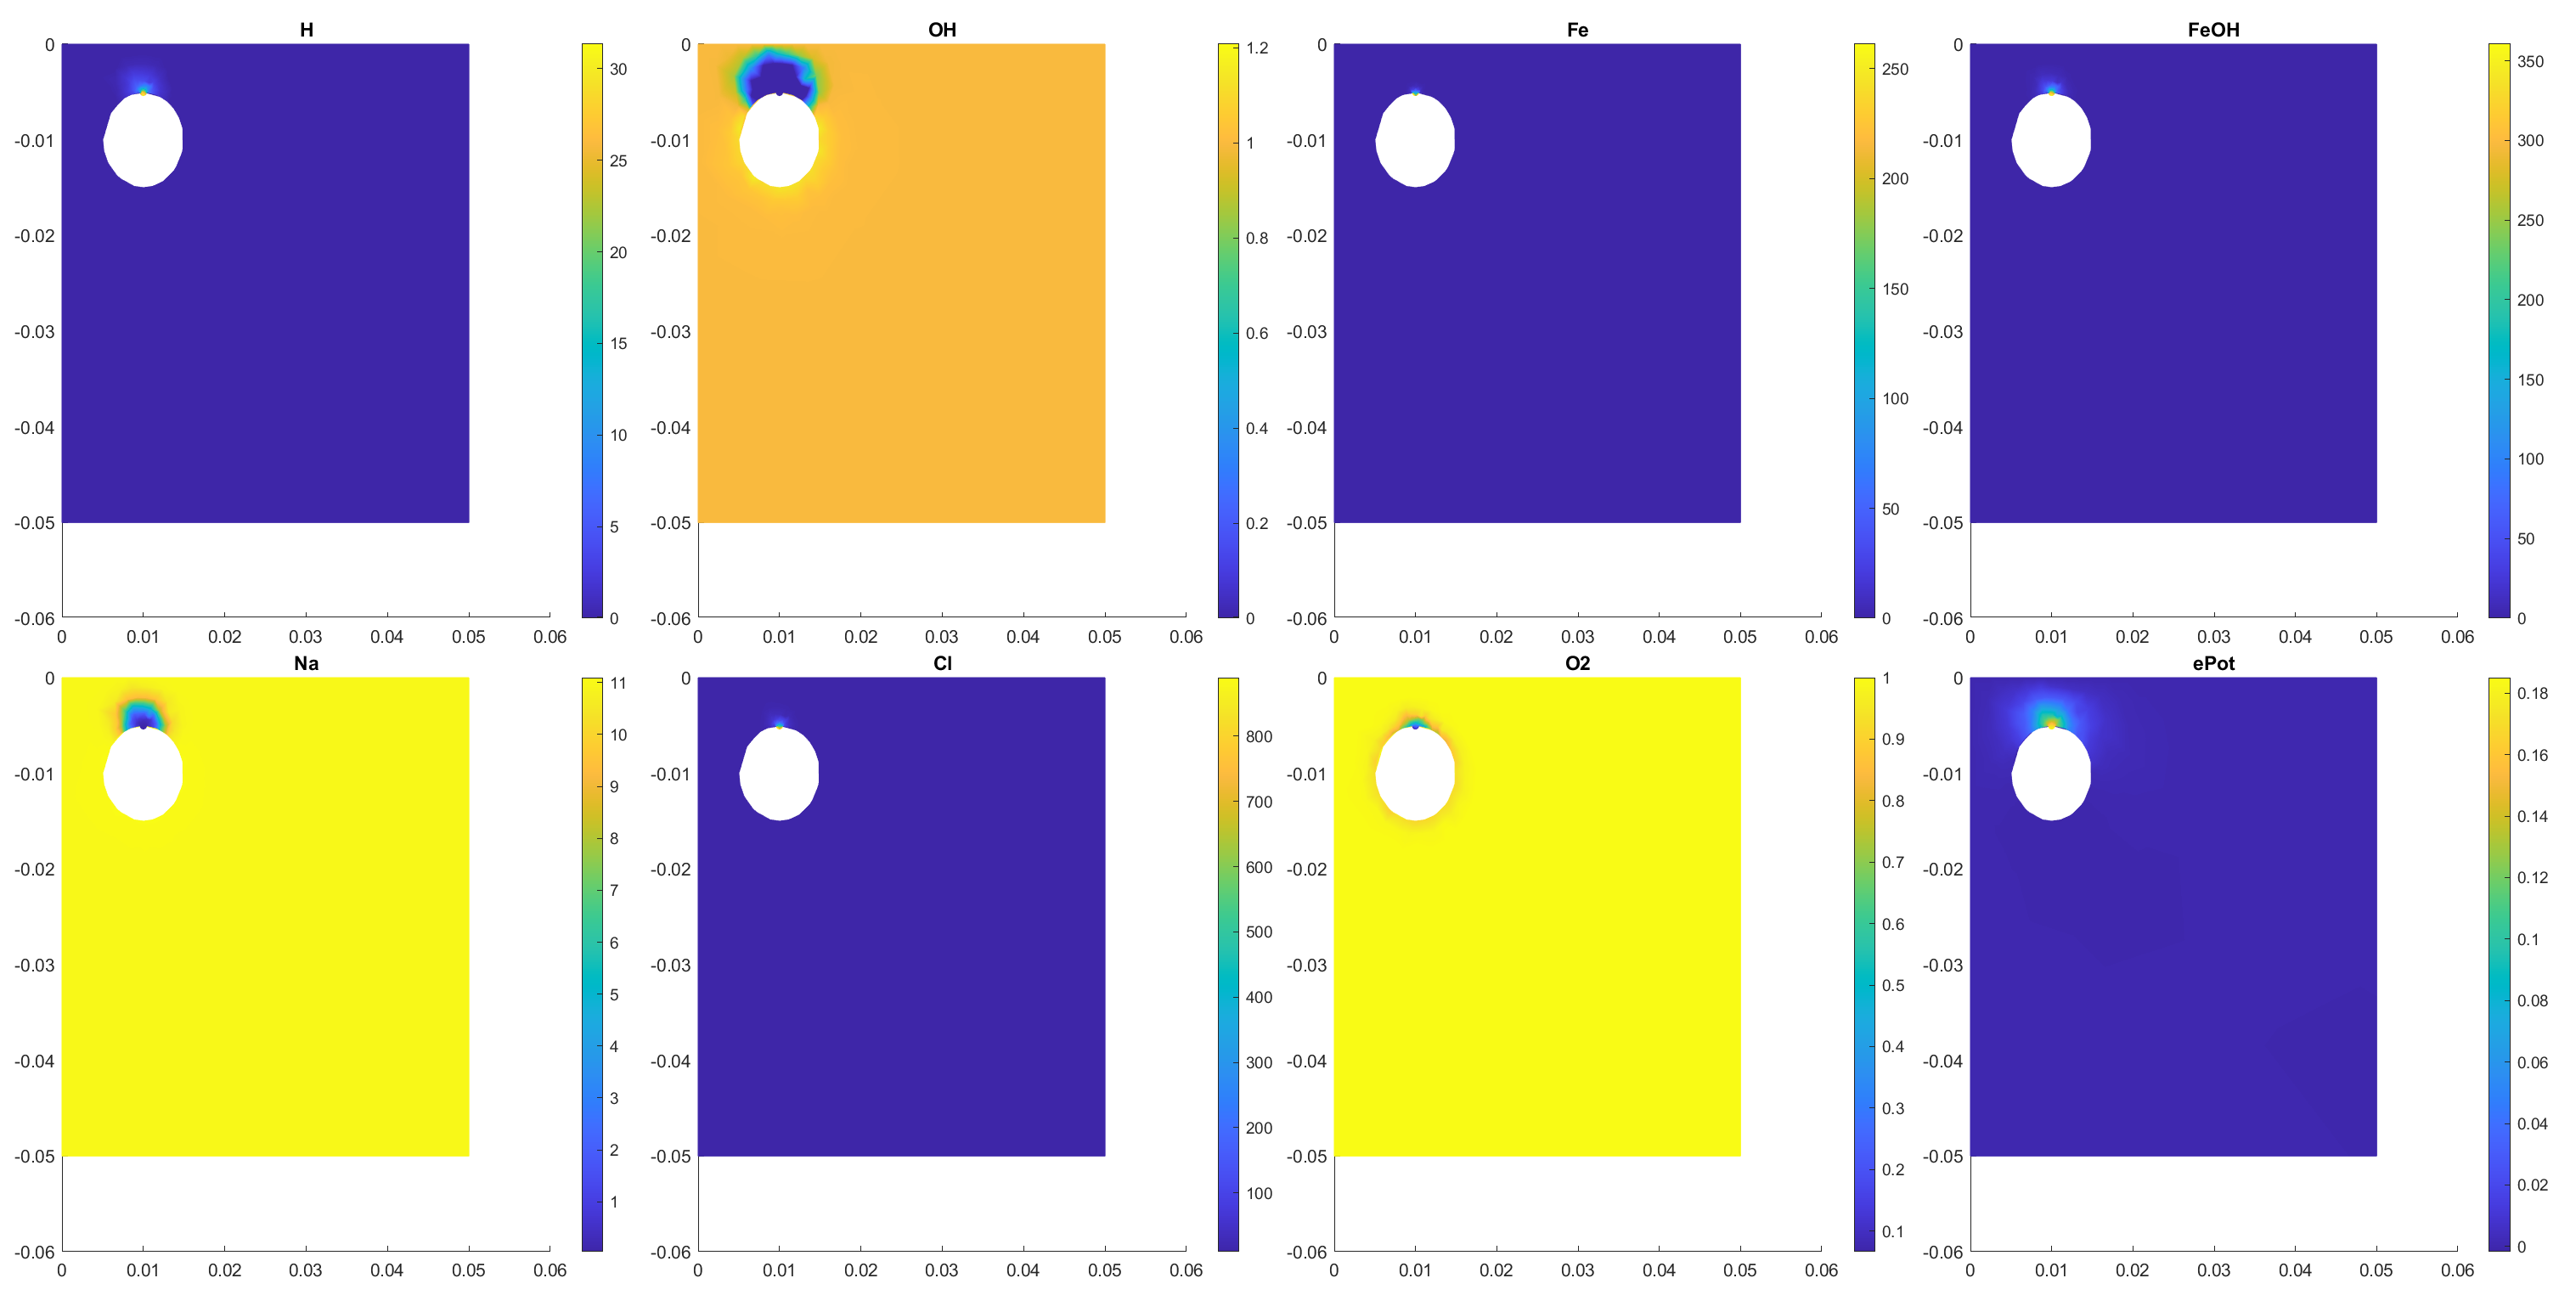
\includegraphics[width=14cm]{PostProcessingA.eps}
	\caption{Example of the post-processing results, showing the concentrations of all species, and the electrolyte potential. }
	\label{fig:PostProcessingA}
\end{figure}

\begin{figure}
	\centering
	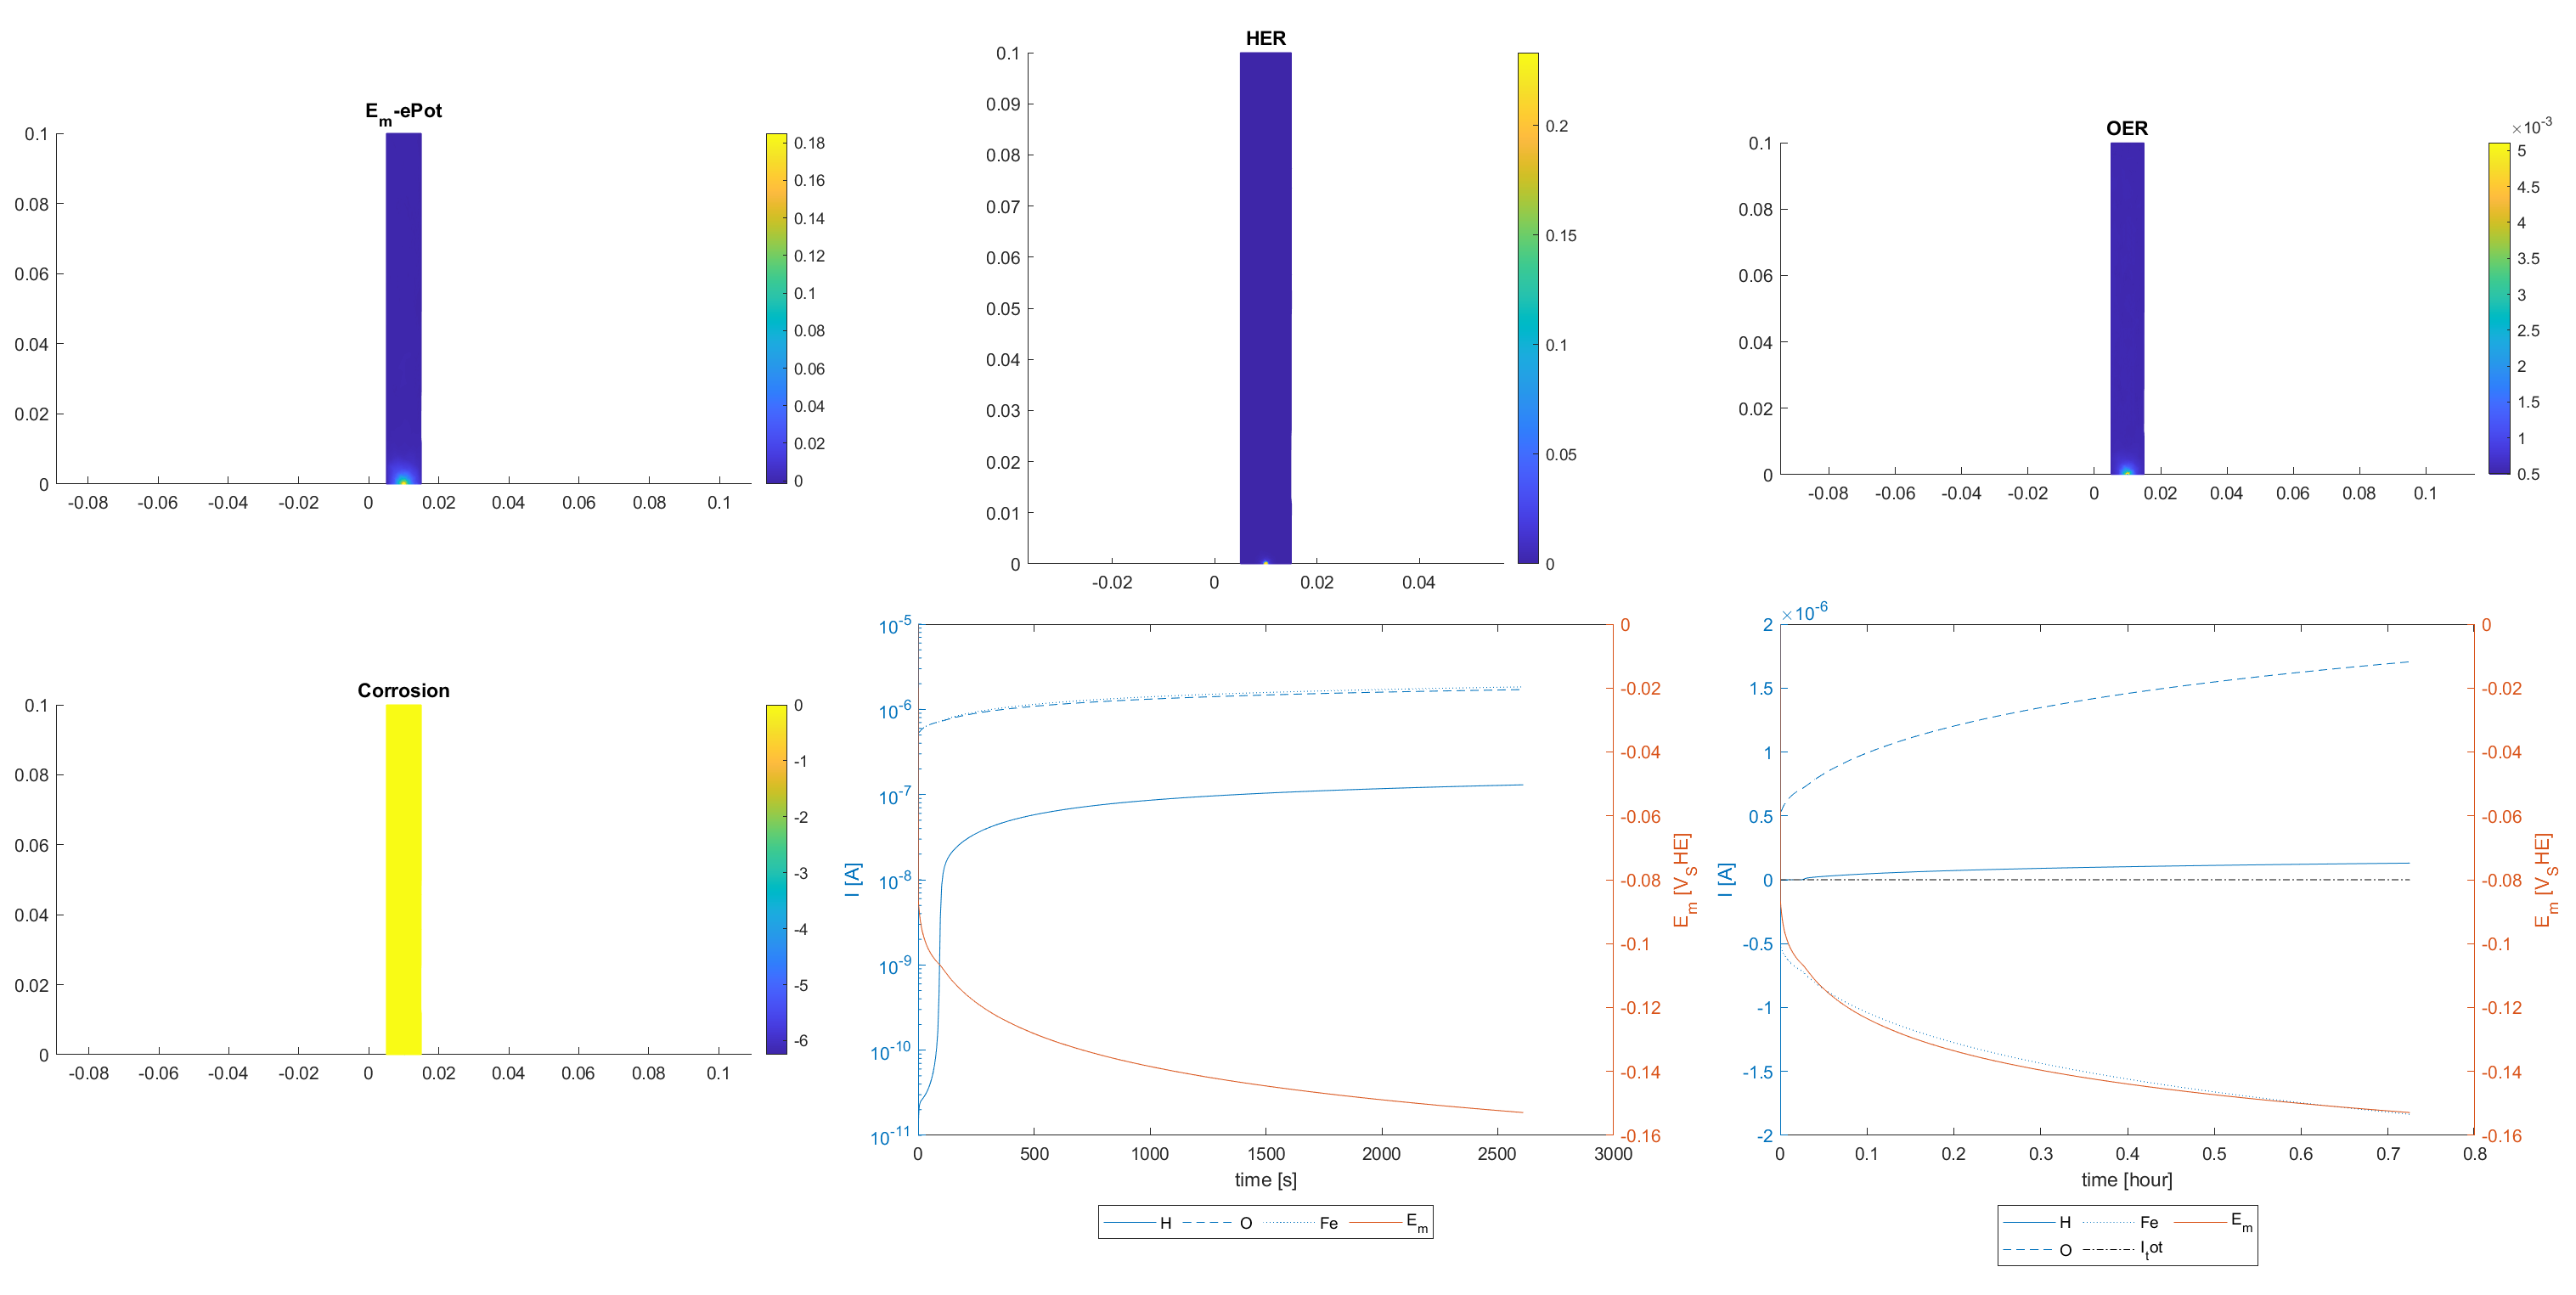
\includegraphics[width=14cm]{PostProcessingB.eps}
	\caption{Example of the post-processing results, showing the surface reaction currents, and the total currents occurring throughout the domain. }
	\label{fig:PostProcessingB}
\end{figure}

The second part of this post-processing script plots the data at the surface of the metal rebar:
\CodeSnipU{TestCases/ElectroChemistry/PlotData_EChem.m}{102}{114}{TestCases/ElectroChemistry/PlotData\_EChem.m}
Producing the results shown in \cref{fig:PostProcessingB}. This shows the surface reaction currents, and the total currents occurring throughout the domain. 

\FloatBarrier
\section{References}
\renewcommand{\bibsection}{}
\bibliography{references}

\end{document}